\section{Návrh a implementácia aplikačného rámca pre IPFIX Mediátor}

Na základe analýzy aplikačného rámca pre sprostredkovanie sprav v IPFIX (pozri kapitolu \ref{sec:framework}, 
strana \pageref{sec:framework}) a analýzy exportovacieho a zhromažďovacieho procesu v RFC 5101
\citep{rfc5101} som zhrnul požiadavky a navrhol samotnú architektúru IPFIX Mediátora. 
Jeho jednotlivým komponentom, ktoré sú vyssie znázornené na obrázku \ref{o:mediator_component_model} 
a požiadavkám sú venované nasledujúce kapitoly. Upozorňujem, že termíny \uv{sprostredkovateľský proces} a 
\uv{modul} sú úplne totožné a zameniteľné.


\subsection{Požiadavky na rámec pre IPFIX Mediátor}

\begin{itemize}
 \item \textbf{Modulárna implementácia} - už počas analýzy sprostredkovania správ v IPFIX bolo zrejmé, že 
 aplikačný rámec musí byť modulárny. Musí mať podporu pre ich jednoduché a flexibilné pridávanie resp. 
 odoberanie. Zdôrazňujem, že predstaviteľom modulu je sprostredkovateľský proces.
 
  \item \textbf{Oddelenie logiky rámca od logiky sprostredkovateľských procesov} - 
  najdôležitejšie je, aby budúci riešitelia sprostredkovateľských procesov nemuseli vôbec zasahovať 
  do zdrojového kódu aplikačného rámca. Všetky potrebné metódy pre prácu so záznamami o tokoch 
  im musí zabezpečiť rámec, ale rovnako im musí zakázať prístup k jeho interným metódam. 
  Iba tak môže byť zachovaná jednotnosť prístupu. Nie je možné, aby každý sprostredkovateľský proces 
  riešil napr. zakódovanie, alebo dekódovanie dátových záznamov po svojom. Preto je potrebné navrhnúť 
  a implementovať rozhranie, prostredníctvom ktorého budú musí  procesy komunikovať s aplikačným rámcom.
  
 \item \textbf{Dynamické načítavanie sprostredkovateľských procesov} - pridávanie a odoberanie 
 sprostredkovateľských procesov musí byť riadené výlučne cez konfiguračný súbor. Nesmie byť potrebný 
 žiadny zásah do zdrojového kódu  rámca.
 
 \item \textbf{Transparentnosť vzhľadom na kolektor} - výstupom Mediátora musia byť správy zakódované 
 v konformite so špecifikáciou IPFIX protokolu. Kolektor spracováva správy prijaté od Mediátora rovnakým
 spôsobom, akoby ich prijal od exportéra.
 
 %% tento dôvod je idiotina :D
 \item \textbf{Komunikácia pomocou UDP} - v tejto fáze projektu som zvolil ako komunikačný protokol UDP.
 Dôvodom bola rýchlosť, jednoduchosť a dobré skúsenosti s implementáciou UDP v JXColl. Napriek tomu, že 
 UDP nie je  spojovo orientovaný transportný protokol, v prípade nasadenia Mediátora v SLAmetri to vôbec
 nevadí. Mediátor bude nasadený fyzicky na tej istej lokálnej sieti ako exportér a kolektor. 
 
 \item \textbf{Jednoduchá konfigurácia} - ako už bolo spomenuté v analýze 
 (kapitola \ref{sec:framework_intermediate}, strana \pageref{sec:framework_intermediate}), 
 sprostredkovateľské procesy spracúvajú prijaté záznamy o tokoch bud sériovo, alebo paralelne. 
 Celková štruktúra odovzdávania dát v rámci mediátora od zhromažďovacieho procesu, sériovo a paralelne cez 
 všetky procesy a napokon až k exportovaciemu procesu musí byť jednoznačne konfigurovateľná v textovom 
 XML súbore a v čo najviac používateľsky priateľskom formáte. 
 
 \item \textbf{Distribúcia dát medzi komponentmi} - aplikačný rámec musí zabezpečiť spôsoby prenosu dát medzi 
 jednotlivými sprostredkovateľskými procesmi a zhromažďovacím a exportovacím procesom. Tieto spôsoby 
 musia byť pre procesy jednotné, transparentné a bez možnosti zmeny z vnútra sprostredkovateľského procesu.
 
 \item \textbf{Jediná inštancia modulov} - navrhol som, že každý sprostredkovateľský
 proces musí byť implementovaný podľa návrhového vzoru \emph{Singleton}. Je to z toho dôvodu, že 
 každý proces musí byť unikátny a jednoznačne rozpoznateľný v rámci celého programu na 
 základe mena triedy procesu. Konfigurácia toku dát cez procesy spomínaná vyššie bude daná práve 
 prostredníctvom názvov ich tried. Jedinečnosť procesov musí zabezpečiť aplikačný rámec. 
 
 \item \textbf{Jednotné dekódovanie a zakódovanie dátových záznamov} - aplikačný rámec musí obsahovať metódy 
 prístupné všetkým sprostredkovateľským procesom, ktoré budú dekódovať dátové záznamy na dáta a opačne
 na základe šablón.
 
 \item \textbf{Viacvláknovosť} - nielen zo samotnej povahy paralelných procesov, ale aj modularity vyplýva, 
 že každý sprostredkovateľský proces bude vykonávaný v samostatnom vlákne, prípadne viacerých vláknach. 
 Podobne zhromažďovací a exportovací proces budú rozdelené na viac vlákien. 
 

 \item \textbf{Konformita s protokolom IPFIX} - zhromažďovací a exportovací proces aplikačného rámca sa 
 nesmú líšiť od charakteristík týchto procesov daných špecifikáciou IPFIX protokolu v RFC 5101 \citep{rfc5101}.
 
 \item \textbf{Programovací jazyk Java} - pre implementáciu som zvolil programovací jazyk Java.
 Hlavným dôvodom bol fakt, že zhromažďovací proces Mediátora a IPFIX kolektora sú veľmi podobné a kolektor 
 JXColl je naprogramovaný v tomto jazyku. Ďalším faktom je relatívne jednoduchá tvorba modulárnych aplikácii,
 vďaka načítavaniu tried pomocou \emph{Java ClassLoader}. V neposlednom rade zohrala svoju rolu aj vysoká
 podpora jazyka Java, či už sa jedná o kvalitu dokumentácie, Veľké množstvo odborných fór, dostupnosť 
 knižníc jazyka, ale aj fakt, že Java aplikácie sú spustiteľné na väčšine operačných systémov.
\end{itemize}

%% -------------------- MEDIATOR -----------------

\subsection{Hlavná trieda Mediátora}


Ulohou hlavnej triedy Mediatora je postupne spustit vsetky vlakna a procesy potrebne pre beh programu.
Najprv sa precitaju a spracuju argumenty prikazoveho riadku. Program vie rozpoznavat dva druhy 
argumentov. Prvym je cesta ku konfiguracnemu suboru. Ak nie je zadana, pouziva sa vychodiskovy 
konfiguracny subor. Druhym argumentom moze byt zadana moznost \verb|--logtofile|. Vtedy su vsetky 
logovacie vystupy presmerovane zo standardneho vystupu do suboru.

Potom ako program nacita vsetky nastavenia z konfiguracneho suboru, spusti vsetky svoje moduly - 
sprostredkovateľské procesy pomocou triedy \verb|IPLoader|. Nasleduje spustenie vlakna, ktore prijima 
IPFIX pakety prostrednictvom protokolu UDP a vlakna, ktore ich spracovava. Hovorime o \verb|UDPServer| 
a \verb|UDPProcessor|. Nakoniec je spustene exportovacie vlakno - \verb|UDPExporter|. Kedykolvek ked 
nastane chyba je Mediator korektne ukonceny a to tak, ze uvolni vsetku pamat a zastavi beziace vlakna. 
Rovnako je Mediator zastavny po stalceni kombinacie klaves \verb|Ctrl+c|.
Podrobne o kazdom spomenutom vlakne a procese bude povedane v nasledujucich kapitolach.






%% -------------------- COLLECTING -----------------

\subsection{Zhromažďovací proces} \label{sec:collectingprocess}

Na základe analýzy a zhodnotenia požiadaviek na zhromažďovací proces som navrhol jeho architektúru.
Logická štruktúra procesu sa skladá z dvoch fáz, pričom každú fázu predstavuje jedno vlákno. 
Venujme sa teda jednotlivým fázam procesu.

\subsubsection{1. fáza zhromažďovacieho procesu}

\begin{figure}[ht!]
\centering
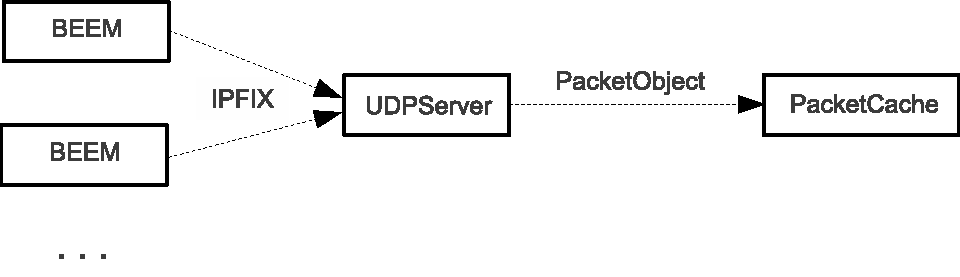
\includegraphics[width=0.8\textwidth]{collecting1_schema}
\caption{Schéma prvej fázy zhromažďovacieho procesu Mediátora}\label{o:collecting1_schema}
\end{figure}

Prvá fáza je znázornená na Obr. \ref{o:collecting1_schema} a predstavuje najnižšiu vrstvu celého 
nástroja. Jej jadrom je UDP server, bežiaci v samostatnom vlákne. V jeho hlavnej metóde \emph{run()}
cyklicky vykonáva kód, dokiaľ nie je prerušený výnimkou \emph{InterruptedException}.
Tento cyklicky kód odchytáva údaje posielané protokolom UDP na úrovni bytov a ukladá ich do 
buffera. K tomuto je použitý objekt triedy jazyka Java - \emph{ByteBuffer}. Zároveň sa do objektu 
triedy \emph{InetSocketAddress} uloží IP adresa exportéra a zaznamená sa čas prijatia dát v 
milisekundách (formát Unix Timestamp). Tieto tri premenné sú argumentom funkcie \emph{write()}, 
ktorá z prijatých premenných vytvorí objekt typu \emph{PacketObject}. Tento objekt je akousi
abstraktnou reprezentáciou paketu, vo svojich členských premenných uchováva údaje z hlavičky
IPFIX správy (sekvenčné číslo, čas exportu, ID pozorovacej domény) spolu s obsahom správy, časom 
prijatia a adresy z ktorej bol prijatý. 
Prijatá IPFIX správa vo forme inštancie triedy PacketObject 
sa uloží do vyrovnávacej pamäte pre správy, ktorú predstavuje trieda \emph{PacketCache}. Jej členská 
premenná \emph{cache} je typu \emph{ArrayBlockingQueue}, čo je vlastne Java implementácia \emph{FIFO}
frontu, ktorý je navyše synchronizovaný a optimalizovaný na vysoký výkon. Tato vyrovnávacia pamäť 
medzi prvou a druhou fázou zhromažďovacieho procesuje kritická vo vysoko rýchlostných sieťach. 

Návrh do budúcnosti umožňuje jednoduché rozšírenie o serveri iných protokolov, napr. TCP a SCTP. 
Tieto serveri budú rovnako ako UDPServer bežiace v samostatných vláknach.

\subsubsection{2. fáza zhromažďovacieho procesu}

\begin{figure}[ht!]
\centering
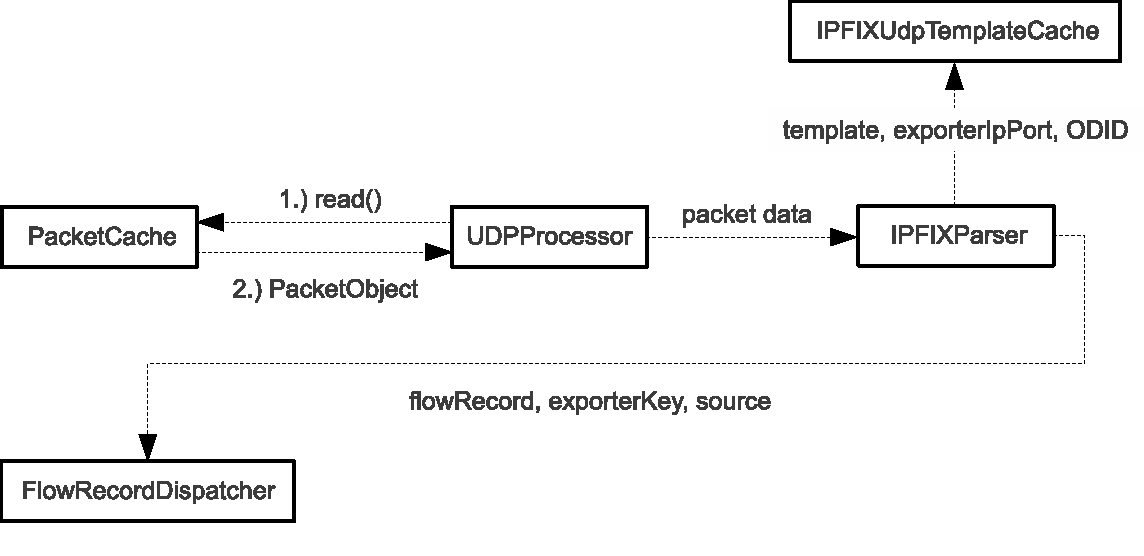
\includegraphics[width=0.8\textwidth]{collecting2_schema}
\caption{Schéma druhej fázy zhromažďovacieho procesu Mediátora}\label{o:collecting2_schema}
\end{figure}

Schému druhej fázy vidíme na Obr. \ref{o:collecting2_schema}. Hlavná metóda \emph{run()} vlákna 
\emph{UDPProcessor} cyklicky vyberá dáta z PacketCache a predáva ich \emph{parseru}, reprezentovaného 
triedou \emph{IPFIXParser}, dokiaľ nie je prerušený výnimkou \emph{InterruptedException} vyhodenou pri 
čítaní z vyrovnávacej pamäte.
UDPProcessor robí zároveň kontrolu, či prijaté dáta sú IPFIX paketom. V tomto prípade, ale aj v prípadoch
keď prijaté dáta sú poškodené sa správa zahadzuje a program pokračuje spracovávaním ďalšej správy z 
vyrovnávacej pamäte.
Trieda \emph{IPFIXParser} sa používa na spracovanie prijatých paketových binárnych dat, ktorého 
výsledkom je hotový objekt IPFIX správy, obsahujúci všetky komponenty správy, pozri kapitolu 
\ref{sec:message_format}, strana \pageref{sec:message_format}. Metódy tejto triedy najprv vykladajú 
kompletnú hlavičku správy a potom sa pustia do parsovania IPFIX sád. Na základe identifikátora sady 
spracujú a vytvoria objekty pre sadu šablón, sadu šablón možnosti a dátovú sadu. Sady následne naplnia 
príslušnými záznamami. 

Prichádzajúce záznamy šablón a záznamy šablón možnosti sú posielané triede 
\emph{IPFIXUdpTemplateCache}, ktorá má na starosti spravu prijatých šablóny osobitne pre každý exportér. 
Ako je zrejme zo špecifikácie exportovacieho procesu, šablóna musí byť odoslaná kolektoru okamžite ako je 
vytvorená a ešte pred odoslaním jej prislúchajúcich dátových záznamov. Potom je šablóna periodicky 
preposielaná. Trieda IPFIXUdpTemplateCache ukladá nove šablóny a objekty šablón, ktoré už má uložené 
aktualizuje. Zároveň maže staré šablóny, ku ktorým nedostala aktualizáciu po dobu definovanú v 
konfiguračnom súbore.

Napokon sa každý dátový záznam v dátovej sade, s prislúchajúcou šablónou a hlavičkou IPFIX správy 
zabalí do objektu triedy \emph{IPFIXFlowRecord}, ktorá je reprezentáciou záznamu o toku. 
Druhým parametrom, ktorý sa posiela triede \emph{FlowRecordDispatcher} je 
reťazec, ktorý určuje odkiaľ záznam vystupuje \emph{(inputProcess)}. V tomto prípade je to 
\emph{\uv{exportér}}. 
Trieda FlowRecordDispatcher rozdistribuuje prijaté záznamy o tokoch príslušným 
sprostredkovateľským procesom, alebo ich pošle na export. O tom podrobnejšie v samostatnej kapitole
\ref{sec:FlowRecordDispatcher}, na strane \pageref{sec:FlowRecordDispatcher}. 

%% -------------------- COLLECTING END -----------------
%% -------------------- INTERMEDIATE -----------------

\subsection{Rozhranie a podpora pre sprostredkovateľské procesy - moduly} \label{sec:intermediate_process}

Vyššie boli definované viaceré požiadavky na sprostredkovateľské procesy, ktorý musí zabezpečiť 
aplikačný rámec. Jedná sa o modulárnu implementáciu, oddelenie logiky rámca od logiky procesov, 
ich dynamické načítavanie, jediná inštancia procesov atď. 

\subsubsection{Java ClassLoader a dynamické načítavanie tried} \label{sec:classLoader}

\emph{Java ClassLoader} je súčasťou \emph{Java Runtime Environment} (JRE) a jeho úlohou je dynamické
načítavanie tried jazyka Java do \emph{Java Virtual Machine} (JVM) na základe ich mena. 
Načítavanie tried je jeden zo základných a najsilnejších mechanizmov, ktorý poskytuje programovací jazyk
Java. Vďaka nemu JRE nemusí vedieť nič o súboroch a súborovom systéme počas vykonávania Java programov. 
Navyše tieto súbory tried nie sú načítavané do pamäte naraz, ale podľa požiadaviek 
programu. \citep{mcmanis, travis}

Načítavanie tried je organizované do stromovej štruktúry. Koreňom štruktúry je samo zavádzací 
\emph{(bootstrap) class loader}, ktorý je napísaný v natívnom kóde a nie je možné vytvárať jeho inštancie. 
Vytvára ho 
JVM a je zodpovedný za načítanie interných tried Java Development Kit (JDK) a \emph{java.*} balíčkov 
obsiahnutých v JVM. Príkladom je \verb|java.lang.String|. Jeho potomkom je \emph{extension class loader},
ktorého primárnou zodpovednosťou je načítavať triedy z \emph{extension} priečinkov. Toto je pohodlný 
spôsob rozšírenia JDK bez pridávania položiek do premenných prostredia - \emph{CLASSPATH}. 
Rozšírením \emph{extension classloader-a} je aplikačný, resp. \emph{systémový class loader}. Jeho úlohou 
je načítanie tried z cesty danej premennou prostredia. Systémový class loader získavame metódou 
\verb|ClassLoader.getSystemClassLoader()|. \citep{techjava, antl}

Abstraktná trieda \verb|ClassLoader| je umiestnená v balíčku \verb|java.lang|. Vývojári môžu pridať 
vlastnú 
funkcionalitu do načítavania tried vytvorením vlastnej, ktorá bude rozšírením triedy 
\verb|ClassLoader|. Typickou stratégiou je transformovanie mena triedy na meno súboru a následné 
prečítanie \uv{súboru triedy} \emph{(class file)} zo súborového systému. \citep{christudas, classloader}

Na dynamické načítavanie tried na základe ich binárneho mena sa používa metóda \verb|loadClass(String name)|.
Tuto metódu som použil pri načítavaní modulov definovaných v konfiguračnom súbore a aj pri získavaní 
inštancii sprostredkovateľských procesov, ktoré boli potrebné pri riadení toku dát medzi procesmi.
Podrobnejšie sa tomu venujem v príslušných kapitolách. 



\subsubsection{Abstraktná trieda AIntermediateProcess} 

Po analýze požiadaviek bolo jasné, že je potrebné pripraviť akési rozhranie pre sprostredkovateľské 
procesy, ktoré by oddeľovalo ich logiku od logiky aplikačného rámca. Navyše toto rozhranie musí 
definovať základné vlastnosti, ktoré sú rovnaké pre všetky procesy a implementovať metódy, ktoré 
majú byť procesom dostupné. Jednoznačnou odpoveďou na tieto otázky je abstraktná trieda, 
od ktorej budú všetky moduly dediť. 


\paragraph{Viacvláknovosť}
Každý modul musí byť vykonávaný v samostatnom vlákne. Preto trieda \emph{AIntermediateProcess} dedi
od triedy \emph{Thread} a obsahuje abstraktnú metódu \emph{run()}, čo je vlastne deklaráciou 
hlavnej metódy vlákien. Toto zabezpečí, že v každom module bude musieť byť jej konkrétna implementácia.


\paragraph{Jediná inštancia modulov} \label{sec:singleton}
Ďalšou požiadavkou bolo, že moduly musia byť implementované podľa návrhového vzoru Singleton. V prípade, že
by existovalo viacero inštancií každého modulu, trieda \emph{FlowRecordDispatcher} by nemohla správne 
distribuovať záznamy o tokoch medzi procesmi. Vzorová implementácia návrhového
vzoru singleton je nasledovná:  
\begin{verbatim}
 public class Singleton {
    private static Singleton instance = null;
 
    private Singleton() {}
 
    public static Singleton getInstance() {
            if (instance == null) {
                   instance = new Singleton();
            }
            return instance;
   }
}
\end{verbatim}
Nedá sa spoľahnúť na to, že budúci vývojári modulov budú implementovať sprostredkovateľské procesy 
podľa tohoto návrhového vzoru, preto to musí zabezpečiť aplikačný rámec, presnejšie trieda od ktorej 
dedia - \emph{AIntermediateProcess}.
Bohužiaľ v jazyku Java nie je možné aby Singleton implementovala abstraktná trieda, hneď z viacerých
dôvodov (vymenované len niektoré):
\begin{enumerate}
 \item Singleton vyžaduje konštruktor s viditeľnosťou \emph{private}. Toto sa vylučuje s možnosťou 
 dedenia.
 \item Členská premenná \verb|instance| je typu \emph{static}. Teda sa viaže k triede Singleton a nie k jej 
 potomkom.
 \item V prípade, že členská premenná \verb|instance| má hodnotu \emph{null}, je potrebné vytvoriť novu inštanciu 
 potomka a nie rodičovskej triedy. Avšak inštanciu ktorého potomka?
 \item Druhý prístup je deklarovať metódu \emph{getInstance()} abstraktnou. Konkrétna implementácia 
 by tak bola zabezpečená triedami sprostredkovateľských procesov, premenná \verb|instance|
 by bola správneho typu. Tento návrh je však nerealizovateľný. 
 Metóda \emph{getInstance()} rodičovskej triedy nemôže byť statická a zároveň abstraktná. V jazyku Java
 to nie je možné \footnote{Niektoré jazyky, napr. Python túto možnosť dovoľujú.}. 
 \emph{Static} metóda patrí triede, kde je definovaná. 
 Pričom \emph{abstract} naznačuje, že funkcionalita bude definovaná až v potomkoch. Tu dochádza k 
 logickému rozporu.
\end{enumerate}
Preto bolo potrebné navrhnúť a implementovať iný spôsob, ktorý by zabezpečil jedinú inštanciu pre všetky 
moduly z abstraktnej rodičovskej triedy. Riešenie navrhol britsky Java programátor Niall Gallagher
na jednom z diskusných fór o probléme dedenia a návrhového vzoru Singleton \citep{gallagher}.
Jeho riešenie je hybridom viacerých prístupov, ktoré sa diskutujú na Internete, no vychádza z 
návrhového vzoru \emph{Factory method}. Výsledkom je abstraktná trieda, slúžiaca ako továreň na 
podtriedy tým, že volá jej statickú metódu \emph{getInstance(Class clazz)}. 
\begin{verbatim}
private static final Map singletonRegistry = new HashMap();

public static final synchronized 
<T extends AIntermediateProcess> T getInstance(Class clazz) {
  T instance = (T) singletonRegistry.get(clazz);
  if (instance == null) {
      try {
          instance = (T) clazz.newInstance();
      } catch (InstantiationException | IllegalAccessException ex) {
          log.error(ex);
      }
      if (instance != null) {
          singletonRegistry.put(clazz, instance);
      } else {
         log.error(Could not register singleton);
      }
 }
 return instance;
}
\end{verbatim}
Ak sú splnené podmienky, že konkrétna trieda, napr. \verb|SelectionProcess| je definovaná v rovnakom 
balíčku ako \verb|AIntermediateProcess| a ich konštruktory nemajú explicitne nastavený prístup 
(predvoleným prístupom je \uv{privátny v rámci balíčka}), tak 
jediným spôsobom ako získať inštanciu podtriedy mimo balíčka je cez konštrukciu:
\begin{verbatim}
 SelectionProcess instance = 
 AIntermediateProcess.getInstance(SelectionProcess.class);
\end{verbatim}
Dalo by sa vyčítať, že vytváranie inštancií používa reflexiu, ktorá je pomalá. Avšak, keďže vytvárame 
Singletony, volanie \emph{newInstance()} sa vykoná pre každý modul pravé raz.

Aby bolo možné získavať inštancie modulov aj na základe mena triedy a nie len cez class objekty, vytvoril 
som ďalšiu metódu \emph{getInstance(String processName)}. Parameter \emph{processName} je práve meno 
procesu, napr \verb|SelectionProcess|. 
Premenná \emph{name} je binárne meno procesu, podľa špecifikácie jazyka Java \citep{java_spec},
napr. \verb|sk.tuke.cnl.Mediator.SelectionProcess|.
Tato metóda načíta \emph{class} objekt sprostredkovateľského procesu cez systémový class loader,
tak ako to bolo vyššie spomínané. Potom zavolá pôvodnú metódu \emph{getInstance(Class clazz)} a 
vráti inštanciu procesu.
\begin{verbatim}
 String name = Default.PROCESSES_LOCATION + processName;
 Class clazz = ClassLoader.getSystemClassLoader().loadClass(name);
 instance = AIntermediateProcess.getInstance(clazz);
\end{verbatim}



\paragraph{Dekódovanie dátových záznamov} 
Bola vyslovená požiadavka, že aplikačný rámec musí obsahovať metódy pre dekódovanie a zakódovanie 
dátových záznamov na základe šablón. Nie je žiadúce, aby v budúcnosti každý vývojár sprostredkovateľských 
procesov riešil tieto úlohy po svojom. 

Už v konštruktori triedy sa získa inštancia triedy \verb|IPFIXElements|, ktorá poskytuje 
funkcie na jednoduché získanie informácii o podporovaných informačných elementoch. Trieda sparsuje XML 
súbor \emph{(ipfixFields.xml)} a dáta uloží do hash mapy, ktorá používa mapovanie z ID informačného 
elementu na objekt typu \verb|IpfixFieldAttributes|. Tento objekt obsahuje informácie o elementoch, ako 
napríklad meno, dátový typ, meno skupiny do ktorej patrí a identifikačné číslo.\citep{veri}

Na dekódovanie slúži metóda \verb|decodeDataRecord(...)|, jej parametrami sú dátový záznam a príslušná
šablóna. V prvej fáze je potrebné získať zakódovanú hodnotu z dátového záznamu, druha fáza dekóduje 
byty informačného elementu na hodnotu definovanú dátovým typom.

V cykle sa prechádzajú všetky špecifikátory poľa v šablóne. Na začiatku procesu sa pre každý 
špecifikátor určí číslo organizácie (ak je definované) a ID informačného elementu. Ak daný informačný
element sa nenachádza v hash mape informačných elementov, tak je zaznamenaná chyba a pokračuje sa 
na spracovanie ďalšieho špecifikátora poľa. Potom sa získa meno, dátový typ a skupina informačného elementu. 
Posledne menované je skôr z informačných dôvodov, kvôli logovacím výpisom. Následne sa určí pozícia 
špecifikátora poľa v šablóne, pretože na rovnakej pozícii je uložená zakódovaná hodnota informačného
elementu v dátovom zázname. Metóda teda získa tieto byty, obalí ich do objektu triedy \emph{ByteBuffer}  
a ten pošle spolu s pomenovaním dátového typu na dekódovanie triede \verb|IPFIXDecoder|.

Autorom tejto triedy je Tomáš Vereščák. Na základe dátového typu je určená metóda, ktorá dekóduje 
byty obsiahnuté v bufferi. Dekódovanie je implementované v súlade s RFC 5101 \citep{rfc5101} a 
RFC 5102 \citep{rfc5102} pre všetky dátové typy podporované protokolom IPFIX. Vymenujem aspoň niektoré:
znamienkové a bezznamienkové celé čísla na 8, 16, 32 a 64 bitoch, čísla v pohyblivej rádovej čiarke na 
32 a 64 bitoch, dátumy, IPv4 a IPv6 adresy, MAC adresy a pod. 

Dekódovaná hodnota je z dekodéra vrátená ako reťazec. Všetky hodnoty sa ukladajú do hash mapy, ktorá 
kvôli jednoduchému vyhľadávaniu prvkov asociuje názov informačného elementu na jeho hodnotu. 
Takáto dátová mapa so všetkými dekódovanými hodnotami z dátového záznamu je vrátená sprostredkovateľskému 
procesu, ktorý si ju vyžiadal.


\paragraph{Zakódovanie dátových záznamov} 
Presným opakom predchádzajúcej metódy je metóda \verb|encodeDataRecord(...)|. Jej parametrami sú dátová 
mapa (výsledok dekódovania), príslušná šablóna a počet polí v dátovom zázname, ktoré je potrebné 
zakódovať - \emph{recordsCount}.

Na začiatku vykonávania metódy sa inicializuje pole objektov \emph{ByteBuffer} o veľkosti recordsCount.
Toto pole slúži ako pomocná premenná pre uchovávanie zakódovaných hodnôt. Zároveň sa vytvorí objekt 
nového dátového záznamu.
Následne sa v cykle prechádzajú všetky hodnoty v dátovej mape. Pri každom prvku sa získa jeho identifikátor
z inštancie triedy \verb|IPFIXElements| na základe mena prvku. Vďaka tomu sa potom dá určiť číslo
organizácie, dátový typ a pozícia špecifikátora poľa v šablóne. 

Keď sú určené všetky potrebné hodnoty, tak dátový typ a hodnota informačného elementu sú poslané triede 
\verb|IPFIXEncoder| na zakódovanie. Tuto triedu som navrhol a implementoval analogicky k dekodéru. 
Aj tu sú pokryté všetky dátové typy, ktoré podporuje IPFIX protokol vrátane jedného naviac - bezznamienkového
celého čísla na 128 bitoch - \emph{unsigned128}. Tento dátový typ využívajú niektoré informačné elementy 
definované Laboratóriom Počítačových Sietí na Technickej Univerzite v Košiciach. Podla špecifikácie
\citep{rfc5101} musia byť zakódované informačné elementy posielané v sieťovom poradí bytov, známom 
tiež ako \emph{Big-Endian}. 

Na základe dátového typu je určená funkcia, ktorá vykoná kódovanie. 
Tieto funkcie musia uskutočniť radu kontrol, či je vstupná hodnota v reťazci validná. 
Pri číselných typoch a dátumoch sa kontroluje správny rozsah a formát čísla, pri MAC adresách zase 
správny formát a podobne.
V prípade, že vstupná kontrola nie je validná, je vyhodená príslušná výnimka a 
kódovanie je úplne ukončené, dátový záznam sa neexportuje. Je neprípustné, aby Mediátor posielal kolektoru
dátové záznamy s prázdnymi hodnotami z dôvodu, že nebolo možné zakódovať hodnotu danú v zlom formáte.  

Pri kódovaní je veľmi dôležitá rýchlosť a pamäťová 
nenáročnosť kódovacích funkcii. Jedna funkcia, napr. na zakódovanie znamienkového celého čísla na 32
bitoch môže byť zavolaná veľakrát v rámci kódovania jediného dátového záznamu. Tento počet zavisí od 
dátových typov informačných elementov v dátovom zázname. Nemusím zdôrazňovať aké množstvo IPFIX paketov 
a dátových záznamov môže Mediátor v čase prijímať. Preto som dával veľký dôraz na to, aby boli 
kódovacie funkcie čo najoptimálnejšie. 

Ukážme si to na príklade. Úlohou je zakódovať znamienkové celé číslo -42 na pole štyroch bytov.
Najjednoduchším a najpohodlnejším riešením je použiť triedu \emph{ByteBuffer}, alokovať pole veľkosti 
4, nastaviť poradie bytov na \emph{Big-Endian}, vložiť číslo -42 a konvertovať na pole 
volaním \verb|array()|. Druhou možnosťou je použiť triedu \verb|BigInteger|, vložiť hodnotu -42, 
a konvertovať na pole bytov. V tejto metóde sa nedá explicitne nastavovať poradie bytov, pole 
je stále zoradené v \emph{Big-Endian}, čo nám vyhovuje. Nepríjemnosťou je dodatočné orezanie na 
potrebný počet bytov. 
\begin{verbatim}
 ByteBuffer buf = ByteBuffer.allocate(4).order(ByteOrder.BIG_ENDIAN);
 byťe[] b1 = buf.putInt(-42).array();
 
 byťe[] b2 = BigInteger.valueOf(-42).toByteArray();
\end{verbatim}
Obe tieto metódy zbytočne pridávajú réžiu, zložitosť a zvyšujú pamäťovú náročnosť výpočtu tým, že 
používajú komplexné Java triedy. Preto som pre všetky konverzie implementoval metódy pomocou bitových
posunov a bitových operátorov. Tieto metódy prevádzajú všetky číselne primitívne typy jazyka Java 
(byte, short, int, long, float a double) na pole bytov. Ukážme si túto konverziu na 4-bytovom 
čísle -42.
\begin{verbatim}
 public static byťe[] intToByteArray(int x) {
        return new byťe[]{
            (byťe) ((x >> 24) & 0xFF),
            (byťe) ((x >> 16) & 0xFF),
            (byťe) ((x >> 8) & 0xFF),
            (byťe) (x & 0xFF)
        };
 }
 
 byťe[] b3 = intToByteArray(-42);
\end{verbatim}

Hodnota zakódovaná na pole bytov sa uloží do pomocného poľa spomínaného vyššie, na rovnakú pozíciu
ako je pozícia špecifikátor poľa v šablóne. Keď sa prejdu všetky hodnoty pripravene na zakódovanie, 
pomocné pole je vykladané v správnom poradí a teda ho môžeme uložiť do objektu dátového záznamu.
Hotový dátový záznam je vrátený sprostredkovateľského procesu, ktorý si ho vyžiadal.


\paragraph{Distribúcia dát medzi modulmi} 
Trieda \verb|AIntermediateProcess| poskytuje rozhranie pre distribúciu záznamov o tokoch medzi 
jednotlivými sprostredkovateľskými procesmi vďaka synchronizovanej metóde \verb|dispatchFlowRecord(...)|. 
Jej jedinou úlohou je zavolanie rovnomennej metódy distribútora záznamov - triedy \verb|FlowRecordDispatcher|.
O tom podrobne v samostatnej kapitole \ref{sec:FlowRecordDispatcher} na strane 
\pageref{sec:FlowRecordDispatcher}.



\subsubsection{Príklad implementácie modulu - ExampleProcess}

Pre budúcich riešiteľov som pripravil jednoduchý príklad implementácie sprostredkovateľského procesu.
Predstavuje ho trieda \verb|ExampleProcess|, ktorej úlohou je veľmi jednoduchá anonymizácia zdrojovej a 
cieľovej IP adresy zmenením čísla posledného oktetu na nulu. 

Trieda demonštruje všetky pravidlá programovania sprostredkovateľských procesov. V prvom rade dedí od 
abstraktnej triedy \verb|AIntermediateProcess|. Taktiež má konštruktor bez explicitne definovaného 
prístupu, v ktorom volá rodičovský konštruktor so svojím menom ako parametrom. Toto síce nie je povinné,
ale zaistí to, že vlákno bude pomenované, teda v príslušných logovacích výpisoch bude jeho meno.
V opačnom prípade dostane vlákno automaticky vygenerované meno \uv{Thread-\emph{n}}, kde n je celé číslo.
Poslednou podmienkou je implementovať hlavnú, štartovaciu metódu vlákien - \emph{run()}.

Trieda \verb|ExampleProcess| zároveň predvádza použitie metód, ktoré poskytuje jej rodičovská trieda.
V cykle čaká na záznamy o tokoch vo svojom vstupnom bufferi \emph{(inputBuffer)} a postupne ich odtiaľ 
číta a odstraňuje. Nazvime ich 
\emph{vstupne záznamy}. Vstupný buffer jej napĺňa trieda \verb|FlowRecordDispatcher|. Po prečítaní 
vstupného záznamu vytvorí a inicializuje \emph{výstupný záznam}. Následne prechádza všetky dátové záznamy
vstupného záznamu, dekóduje ich, anonymizuje zdrojovú a cieľovú IP adresu a naspať zakóduje. Ak všetko 
prebehlo bez problémov, tak dátový záznam priradí výstupnému záznamu. Napokon výstupný záznam o toku 
posunie distribútorovi záznamov, ktorý ho bude prepošle 
nasledujúcemu sprostredkovateľskému procesu, alebo pripraví na export.

\subsubsection{Dynamické načítavanie sprostredkovateľských procesov} \label{sec:intermediate_load}

Bola definovaná požiadavka, že sprostredkovateľské procesy musia byť načítavané dynamicky, bez nutnosti
zásahu do zdrojového kódu aplikačného rámca. 

Administrátori definujú zoznam procesov v XML konfiguračnom súbore, v elemente \verb|<processes>|. 
Tato položka sa skladá z ďalších položiek typu \verb|<process>| s atribútom 
obsahujúcim meno sprostredkovateľského procesu. Každý proces, ktorý má byť načítaný, musí mať 
samostatnú položku. Príklad takejto konfigurácie uvediem v nasledujúcej kapitole \ref{sec:FlowRecordDispatcher}.

Parser konfiguračného súboru spracuje tieto položky a vytvorí zoznam modulov, ktoré sa majú načítať.
Dynamické načítavanie tried podľa ich mena bolo analyzované v kapitole \ref{sec:classLoader} na strane
\pageref{sec:classLoader}. Načítavanie modulov má na starosti trieda \verb|IPLoader|. Jej hlavná metóda
\verb|loadProcesses()| cyklicky prechádza zoznam reťazcov obsahujúcich názvy modulov. Meno každého 
modulu prevedie na binárny názov a vďaka \emph{systémovému class loader}-u, získa jeho 
\emph{class objekt}. Podmienkou, však je, že hlavná trieda modulu musí byť v rovnakom balíčku ako trieda
\verb|AIntermediateProcess|. Ta potom pomocou metódy \verb|getInstance(...)|, podrobne rozpísanej vyššie, 
získa jedinečnú inštanciu sprostredkovateľského procesu. Keďže každý proces je samostatným vláknom, teda 
dedí od triedy \verb|Thread|, už ho len ostáva spustiť pomocou metódy \verb|start()|. Toto zabezpečí 
reflexia, ktorá získa metódu a následne ju vyvolá \emph{(invoke)}.
\begin{verbatim}
 Object instance = AIntermediateProcess.getInstance(clazz);
 Method start = clazz.getMethod("start");
 start.invoke(instance);
\end{verbatim}

Ak pri načítavaní modulov nenastane žiadna chyba, pokračuje sa v ďalšom vykonávaní programu. V opačnom 
prípade, hoci ak len jeden proces nebol úspešne načítaný, je program Mediátor ukončený.


%% -------------------- INTERMEDIATE END -----------------
%% -------------------- FLOWRECORD DISPATCHER -----------------


\subsection{Trieda FlowRecordDispatcher} \label{sec:FlowRecordDispatcher}

\begin{figure}[ht!]
\centering
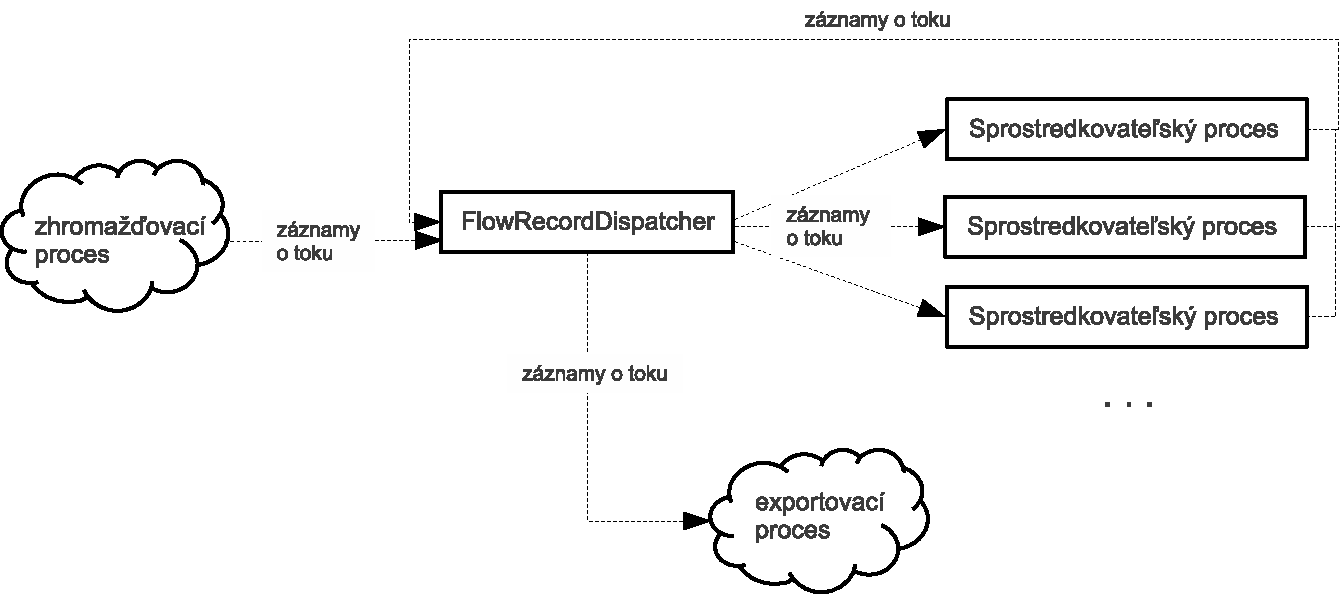
\includegraphics[width=0.9\textwidth]{flowRecordDispatcher_schema}
\caption{Schéma toku dát cez triedu FlowRecordDispatcher}\label{o:flowRecordDispatcher_schema}
\end{figure}

Úlohou tejto triedy je riadiť tok dát medzi komponentami IPFIX Mediátora na základe nastavenia v 
konfiguračnom súbore.
Ukážme si príklad takejto konfigurácie:
\begin{verbatim}
<processes>
        <process name="SelectionProcess">
            <input>exporter</input>
        </process>
        <process name="AggregationProcess">
            <input>exporter</input>
        </process>
        <process name="AnonymizationProcess">
            <input>AggregationProcess</input>
        </process>
</processes>
\end{verbatim}

Majme 3 sprostredkovateľské procesy: 
\begin{itemize}
\item SelectionProcess
\item AggregationProcess a 
\item AnonymizationProcess 
\end{itemize}

Formát zápisu toku dát medzi procesmi je rovnaký ako v príklade. Vstupnými údajmi pre 
\emph{SelectionProcess} a \emph{AggregationProcess} sú dáta priamo prijaté od exportéra, teda sú 
vlastne výstupnom  
zhromažďovacieho procesu. Pričom vstupnými údajmi pre \emph{AnonymizationProcess} je výstup 
z \emph{AggregationProcess}. Tie procesy, ktorých dáta nevstupujú do žiadneho iného sprostredkovateľského 
procesu sú logicky \uv{koncovými} procesmi, ich výstup je posunutý exportovaciemu procesu a poslaný 
kolektoru. Kým pri SelectionProcess a AggregationProcess hovorime o paralelnom spracovaní, 
AnonymizationProcess spracováva záznamy sériovo.

Úloha triedy FlowRecordDispatcher začína keď prijme prvé dáta od zhromažďovacieho procesu. Dáta prijíma 
cez nasledujúce dva 
parametre: záznam o toku - \emph{IPFIXFlowRecord} a reťazec určujúci odkiaľ tento záznam vystupuje - 
\emph{inputProcess}.
Následne získa zoznam prijímateľov tohto záznamu o toku, teda tie sprostredkovateľské procesy, 
ktorých položkou \emph{$<$input$>$} v konfiguračnom súbore je reťazec \emph{inputProcess}, v tomto 
prípade \uv{exportér}. Pri konfigurácii ako je daná v príklade by zoznam obsahoval dva reťazce: SelectionProcess
a AggregationProcess. Teraz potrebujeme získať inštancie týchto tried a ich vstupným bufferom poslať 
prijatý záznam o toku. FlowRecordDispatcher to vykoná v cykle. 
Metódou \emph{getInstance(String processName)} zavolanou nad
abstraktnou triedou \emph{AIntermediateProcess} získa jedinú inštanciu sprostredkovateľského procesu. 
Tato metóda nie je triviálna, podrobne som sa jej venoval v časti 
\emph{Jediná inštancia modulov} na strane \pageref{sec:singleton}. Každej takto získanej 
inštancií sprostredkovateľského procesu zapíše do vstupného buffera \emph{inputBuffer} záznam o toku.

Vstupný  buffer implementuje trieda \verb|IPInputBuffer|, ktorá je analógiou k triede \verb|PacketCache|.
Samotnú buffer rovnako predstavuje synchronizovaný a vysoko výkonný \emph{FIFO} front, implementovaný 
pomocou \verb|ArrayBlockingQueue|. Do cache sú zapisované objekty typu \verb|IPFIXFlowRecord|.

Sú tri základne metódy, s rôznymi parametrami, ktoré zapisujú do frontu.
Metóda \verb|offer()| vloží objekt na koniec frontu, iba v prípade, že je to možné 
okamžite bez prevýšenia kapacity frontu a vráti \emph{true} ak bol zápis úspešný, \emph{false} v 
opačnom prípade. Tato metóda sa viac preferuje ako \verb|add()|, ktorá pri neúspešnom zápise 
vyhodí výnimku. Treťou je metóda \verb|put()|. Jej špecialitou je to, že v prípade, že je front plný,
čaká na uvoľnenie miesta. Toto však spôsobí zablokovanie celého vlákna. \citep{arrayblockingqueue}

V zhromažďovacom procese, v kapitole \ref{sec:collectingprocess} na strane \pageref{sec:collectingprocess},
sa do frontu zapisuje metódou \verb|put()|. V prípade, že sa \emph{PacketCache} naplní, je na mieste 
zablokovať \emph{UDPServer} a počkať a uvoľnenie miesta vo vyrovnávacej pamäti. Avšak na tomto mieste by 
to nebolo vhodné. Stačilo by, že by jeden sprostredkovateľský proces nestíhal spracovávať svoje záznamy
o tokoch, zablokovalo by to dispečera tokov a tým cele vlákno predstavujúce druhú fázu zhromažďovacieho
procesu. Kvôli jednému procesu, by žiaden proces nedostával nové záznamy. Preto zápis do vstupného buffera
sprostredkovateľských procesov zabezpečuje metóda \verb|offer()|.

Ak metóda na získanie zoznamu prijímateľov vráti prázdny zoznam, vyplýva, že záznam o toku 
sa nemá presmerovať ďalšiemu sprostredkovateľskému procesu, ale je už určený na export. Preto záznam o 
toku je zapísaný do vyrovnávacej pamäte pre export. Výsledkom je, že dáta boli presmerované správnym 
prijímateľom a boli splnené príslušné požiadavky na rámec pre IPFIX Mediátor.

%% ----------- FLOWRECORD DISPATCHER END ---------
%% -------------------- EXPORTING -----------------
\subsection{Exportovací proces}

Poslednou fázou Mediátora je exportovací proces. Jeho schéma je zobrazená na obrázku 
\ref{o:exporting_schema}. Ako bolo povedané v predchádzajúcej kapitole, záznamy 
o tokoch, ktoré sú výstupom \uv{koncových} sprostredkovateľských procesov sú prostredníctvom dispečera 
tokov pripravené na export zapísaním do exportovacej pamäte.

\begin{figure}[ht!]
\centering
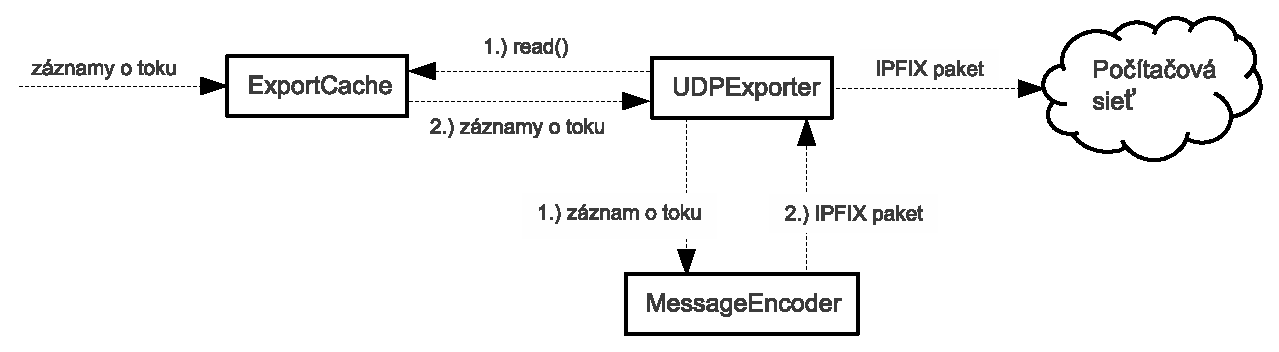
\includegraphics[width=0.8\textwidth]{exporting_schema}
\caption{Schéma exportovacieho procesu}\label{o:exporting_schema}
\end{figure}

Exportovaciu pamäť predstavuje trieda \verb|ExportCache|. Tá je rovnako ako \emph{PacketCache} a 
\emph{IPInputBuffer} synchronizovaný \emph{FIFO} front, do ktorého sa zapisujú objekty typu 
\verb|IPFIXFlowRecord|. Ak sa \verb|ExportCache| naplní, sprostredkovateľské procesy nemajú byť blokované, 
ale pokračovať vo svojej práci. Preto sa do cache zapisuje metódou \verb|offer()|.

Jadrom exportovacieho procesu je trieda \verb|UDPExporter|, predstavujúca samostatné vlákno. V 
konštruktori vytvára UDP soket na prijímanie a posielanie paketov a naviaže ho na akýkoľvek voľný port.
K tomu slúži volanie bezparametrického konštruktora triedy \verb|DatagramSocket|. V jeho hlavnej metóde 
\verb|run()| vykonáva cyklus dokiaľ nie je prerušený. V cykle číta a vyberá záznamy o tokoch z 
vyrovnávacej pamäte pre export. Záznamy posiela triede \verb|MessageEncoder|, ktorá z neho poskladá 
IPFIX paket.

\verb|MessageEncoder| vo svojich metódach postupne tvori obsah IPFIX správy podľa formátu, ktorý som 
analyzoval v kapitole \ref{sec:message_format} na strane \pageref{sec:message_format}. Najprv vypočíta 
sekvenčné číslo, ktoré je obsahom hlavičky každej správy. Toto číslo zodpovedá celkovému počtu doteraz 
odoslaných dátových záznamov modulo $2^{32}$. Ich celkový počet si priebežne zvyšuje vo svojej členskej 
premennej. Potom postupne kóduje sady šablón, dátové sady, určí, resp. vypočíta všetky položky 
hlavičky správy a napokon všetko pospája do výslednej správy.

Trieda rozhoduje, či v posielanej IPFIX správe má byť zahrnutá aj šablóna prislúchajúca dátovým záznamom
obsiahnutým v zázname o toku z ktorého vytvára spravu. Každá šablóna vo svojej členskej premennej uchováva
čas, kedy bola posledne exportovaná. Ak rozdiel medzi prítomnosťou a časom posledného exportu je väčší ako 
je hodnota \verb|<ipfixTemplateTimeout>| definovaná v konfiguračnom súbore, tak šablóna musí byť pripojená.
Rovnako je šablóna pripojená okamžite po jej aktualizácii exportérom. 

Metóda na zakódovanie šablóny používa objekt triedy \verb|ByteArrayOutputStream|. Táto trieda 
implementuje prúd údajov, v ktorom sú dáta zapisované do poľa bytov. Do tohto prúdu postupne kóduje údaje 
v takom poradí ako definuje formát IPFIX správy. Najprv do prúdu zakóduje číslo šablóny, za ním 
počet špecifikátorov poľa a potom samotné špecifikátory. Formát špecifikátorov je nasledovný. Ako prvé sa 
kóduje číslo informačného elementu na dvoch bytoch. V prípade, že ide o element definovaný 
spoločnosťou, tak najvyšší bit sa nastaví na 1. Nasleduje dĺžka informačného elementu a v prípade potreby 
číslo spoločnosti definované organizáciou IANA. Keď je prúd záznamu šablóny hotový, tak sa pred neho 
zaradia zakódované údaje sady šablóny. Tie pozostávajú z čísla sady, čo je v prípade sady šablóny číslo 2
a celkovej dĺžky záznamu šablóny 
vrátane veľkosti hlavičky sady. Touto operáciou vznikne prúd bytov sady šablóny.

Po zakódovaní šablóny sa postupne kódujú všetky dátové záznamy obsiahnuté v zázname toku. Jednotlivé 
hodnoty polí už sú správne zakódované podľa dátového typu, toto majú na zodpovednosti sprostredkovateľské
procesy. Takže v tejto fáze stačí cyklicky prejsť všetky dátové záznamy a ich zakódované polia zapísať 
do prúdu bytov. Napokon je potrebné pred tento prúd bytov zaradiť zakódované údaje dátovej sady. Konkrétne
ide o číslo prislúchajúcej šablóny a súčet dĺžok všetkých dátových záznamov vrátane veľkosti hlavičky sady.
Takto je vytvorený prúd bytov dátovej sady.

Ako posledný sa zostaví prúd bytov hlavičky IPFIX správy. Dĺžka správy je určená súčtom veľkosti hlavičky
správy s veľkosťou sady šablóny a dátovej sady. Ako prvé sa do prúdu bytov hlavičky zakóduje číslo 
verzie, teda \verb|0x000a| a dĺžka správy. Nasleduje čas exportu, vypočítané sekvenčné číslo a ID 
pozorovacej domény, ktoré je nastavené administrátorom v konfiguračnom súbore. Toto číslo však definuje
pozorovaciu doménu v ktorej sídli Mediátor, nie exportér. O určovaní času exportu podrobnejšie neskôr.

V analýze som uviedol implementačno-špecifické problémy Mediátora, kapitola \ref{sec:problems}, strana 
\pageref{sec:problems}. Prvým bola strata informácii o pôvodnom exportéri. Ako som uviedol neskôr, v analýze
exportovacieho procesu v kapitole \ref{sec:exporting_process}, na strane \pageref{sec:exporting_process},
spôsobom ako posielať tieto informácie je zakódovať ich do informačných elementov skupiny 2. Na požiadavku
mediátora boli všetky informačné elementy z tabuľky \ref{t:ie-group2} implementované na strane exportéra.
ID pozorovacieho bodu a pozorovacej domény v ktorej sídli exportér sa kolektor dozvie z príslušných 
informačných elementov, ktoré taktiež exportér podporuje. 

Druhým problémom bola strata informácie o čase exportu. RFC 6183 \citep{rfc6183} popisuje dva spôsoby 
určenia času exportu:
\begin{enumerate}
 \item Zachovávať hodnotu z hlavičky prichádzajúcich IPFIX správ.
 \item Nastaviť aktuálnu hodnotu času keď IPFIX správa opúšťa Mediátor.
\end{enumerate}
V prípade, že exportér posiela akýkoľvek \uv{\emph{delta-}} informačný element, napr. \emph{flowStartDeltaMicroseconds},
tak musí byť použitý prvý spôsob určenia času exportu. Aby Mediátor vyhovoval obom prípadom, navrhol som,
že spôsob určovania času exportu definuje administrátor v konfiguračnom súbore, v elemente \verb|<exportTime>|. 
Ak zadá reťazec \verb|KEEP|, tak trieda \verb|MessageEncoder| zakóduje do prúdu bytov hlavičky pôvodnú
hodnotu. V prípade reťazca \verb|RENEW| sa zakóduje aktuálna hodnota.

Poslednou úlohou triedy \verb|MessageEncoder| je pospájať jednotlivé prúdy bytov do výsledného prúdu IPFIX 
správy. Prvým je prúd bytov hlavičky správy. Ak sa exportuje aj šablóna, tak nasleduje prúd sady šablóny 
a posledným je prúd dátovej sady. Trieda \verb|UDPExporter| teraz z prúdu IPFIX správy vytvori 
UDP paket. Na to slúži trieda \verb|DatagramPacket|, pričom jej parametrami sú dáta, dĺžka správy, 
IP adresa a UDP port. Posledné dve menované sú zadané administrátorom v konfiguračnom súbore. Metódou 
\verb|send()| zavolanou nad soketom je správa odoslaná.






